% @119: Introduction
% =====================================================
The most used framework for \textit{ab initio} calculations, Density 
Functional Theory (DFT) within the Local Density Approximation (LDA),
\cite{kohnPR65} underestimates the energy band gap of semiconductors. It is 
well understood that one has to include the many-body interaction to correct 
for this underestimation of the gap. In this context, the so-called GW 
approximation\cite{onidaRMP02} is known to correct the electronic gap of most 
semiconductors\cite{luceroJPCM12}. However this can be a very expensive
calculation and thus one uses the much simpler scissors operator scheme.
\cite{levinePRL89,levinePRL91,delsolePRB93}  
This allows us to ``open'' the DFT-LDA gap to 
its correct experimental or GW value for most bulk semiconductors.
%%%% Valerie and Nicolas remove these lines
% even when experiments are not available. 
%%%%
This approximation has already been used in linear optical calculations for 
surfaces, see \cite{kippPRL96}, thus improving the agreement with 
experimental results. 
In this context, to correct for the underestimation of the energy band gap of 
semiconductors Nastos et al.\cite{nastosPRB05} used the ``length gauge'' or 
``$\mathbf{r}\cdot\mathbf{E}$ gauge'' to show how to correctly include the 
many-body corrections through the scissors operator in the SH susceptibility.
Later, Cabellos \textit{et al}.\cite{cabellosPRB09} elaborated a derivation 
of the ``velocity gauge'' or ``$\mathbf{A}\cdot\mathbf{v}$'' gauge properly including the 
scissors operator and proved gauge invariance with respect to the length 
gauge. From these works it is clear the length gauge is a much better starting
point to obtain the surface SH (SSH) susceptibility, as will be elaborated 
in this article. However, these considerations are only valid for bulk 
semiconductors.

% =====================================================




% @1192: Half-slab vs. full-slab
% =====================================================

In Fig.~\ref{fig2}
we compare 
$\chi^{xxx}_{\mathrm{half-slab}}$  
vs. 
$\chi^{xxx}_{\mathrm{full-slab}}$ 
for the four different possibilities 
between including or not including the
effects of $\mathbf{v}^\mathrm{nl}$ or the scissors correction
$\hbar\Delta$.   
For these results we chose
$\hbar\Delta=0.5$ eV, that is the GW gap reported in
Refs.~\onlinecite{rohlfingPRB95,garciaCPC01}. 
This is justified by the fact that the surface states of the clean 
Si(001) surface investigated are found, from GW calculations 
\cite{rohlfingPRB95}, to shift rigidly and to keep their dispersion with 
respect to LDA.
We see that for all four instances the 
difference between responses is quite small.
Indeed, when the value $|\chi^{xxx}|$ 
is large the difference between the two is very small; 
when the value is small the difference increases only slightly, 
but the spectra is so close to zero that it is negligible. 
These differences would decrease as the number of atomic layers 
increases. We remark that 32 layers in the slab is more than enough 
to confirm that the extraction of the surface second-harmonic 
susceptibility from the $2\times 1$ surface is readily possible 
using the formalism contained in Eq.~\eqref{chis}.
We have confirmed that for the dihydride surface
$|\chi^{xxx}_{\mathrm{half-slab}}|\approx 0$ (not shown).
This confirms the validity of our theory and is the main result of
this article; through the proposed layer formalism we can calculate the surface SH
$\chi^{\mathrm{a}\mathrm{b}\mathrm{c}}(-2\omega;\omega,\omega)$    
including
the
contribution of the nonlocal part of the pseudopotentials 
and the part of the many-body effects through the scissors correction.
Our scheme should work for any slab.

% =====================================================




% @409: Length Gauge Formalism
% =====================================================

According to ~\onlinecite{ismailPRL01}, we first start with the interaction 
Hamiltonian expressed in the velocity gauge, containing the nonlocal parts
$V^{nl}$ and $S$. Within the dipole approximation and using a gauge 
transformation, it can be transformed into an effective Hamiltonian 
\cite{Veniard, unpublished}
\begin{equation}
H_{I}(t)=-e\mathbf{r}\cdot \mathbf{E}(t).
\label{rde}
\end{equation}
The treatment of the position operator $\mathbf{r}$ for extended Bloch states 
is problematic and has been discussed in Refs.\cite{adamsJCP53,blountSSP62}
%%%% Valerie and Nicolas remove these lines
% In particular, Ref.~\onlinecite{aversaPRB95} develops the treatment of 
% $\mathbf{r}$ for the calculation of the nonlinear optical response.
%%%%
Following Ref.~\onlinecite{sipePRB00} we take the
matrix elements of Eq.~\eqref{rhop} with the $H_{I}(t)$ of 
Eq.~\eqref{rde}, we obtain 
$(\tilde{\rho}^{(1)}(t))_{nm}=B_{nm}^{b}E^{b}(\omega)e^{i(\omega^\Sigma_{nm}-\tilde\omega)t}$,
with 
\begin{equation}
B_{nm}^{b}=\frac{e}{\hbar }\frac{f_{mn}r_{nm}^{b}}{\omega^\Sigma_{nm}-\tilde\omega},
\label{j.1}
\end{equation}
and 
\begin{equation}
(\tilde{\rho}^{(2)}(t))_{nm} = \frac{e}{i\hbar }\frac{1}{\omega^\Sigma_{nm}-2\tilde\omega}\bigg[
i\sum_{q }\Big(r_{nq }^{b}B_{q m}^{c}-B_{nq}^{c}r_{q m}^{b}
\Big)  
-(B_{nm}^{c})_{;k^{b}}\bigg]E^{b}(\omega)E^{c}(\omega)e^{i(\omega^\Sigma_{nm}-2\tilde\omega)t}
.
\label{j.2}
\end{equation}
$\mathbf{r}$ is split into the {\it intraband} 
($\mathbf{r}_i$) and {\it interband} ($\mathbf{r}_e$) parts, where 
$\mathbf{r}=\mathbf{r}_i+\mathbf{r}_e$. 
For $\mathbf{r}_e$ one uses
\begin{equation}
\langle n\mathbf{k} | \mathbf{r}_e | m\mathbf{k}'\rangle =
(1-\delta_{nm})\delta(\mathbf{k}-\mathbf{k}')\boldsymbol{\xi}_{nm}(\mathbf{k})
,
\label{rnminn}
\end{equation}
such that $\mathbf{r}_{e,nm}=0$ for $n=m$.
From Eq.~\eqref{mv} with $H_0\to
H^\Sigma_0$, we obtain
\begin{align}
\mathbf{r}_{e,nm}(\mathbf{k}) =
\boldsymbol{\xi}_{nm}(\mathbf{k})\equiv 
\mathbf{r}_{nm}(\mathbf{k}) 
&=
\frac{\mathbf{v}^\Sigma_{nm}(\mathbf{k})}{i\omega^\Sigma_{nm}(\mathbf{k})}
\quad\quad n\notin D_m 
,
\label{pmnrmn}
\end{align}  
where we defined
$\omega^\Sigma_{nm}(\mathbf{k})\equiv\omega^\Sigma_n(\mathbf{k})-\omega^\Sigma_m(\mathbf{k})$, and
$D_m$ are all the possible degenerate $m$-states. 
For the intraband part, $\mathbf{r}_i$ only appears in
commutators during the derivation of
the optical response. We use,\cite{aversaPRB95}
\begin{equation}
\langle n\mathbf{k} | [\mathbf{r}_i,{\cal O}] | m\mathbf{k}'\rangle
=i\delta(\mathbf{k}-\mathbf{k}')({\cal O}_{nm})_{;\mathbf{k}},
\label{conmri3n}
\end{equation}  
where
\begin{equation}
({\cal O}_{nm})_{;\mathbf{k}}=
\nabla_\mathbf{k} 
{\cal O}_{n m}(\mathbf{k}) 
- 
i 
{\cal O}_{nm}(\mathbf{k}) 
\left(
\boldsymbol{\xi}_{nn}(\mathbf{k}) 
-
\boldsymbol{\xi}_{mm}(\mathbf{k}) 
\right) 
,
\label{gendevnn}
\end{equation} 
is
the generalized derivative 
of the operator ${\cal O}$. 
The vectors $\boldsymbol{\xi}_{nn}(\mathbf{k})$ are defined in 
Ref.~\onlinecite{aversaPRB95} though they do not need to be 
calculated explicitly in what follows. 

Before continuing,
we derive a key result for the length gauge formulation. 
Again, using $H^\Sigma_0$ in
Eq.~\eqref{mv} we obtain
\begin{align}
\mathbf{v}^\Sigma&=
\mathbf{v} 
+
\mathbf{v}^\mathrm{nl} 
+\mathbf{v}^S
=
\mathbf{v}^\mathrm{LDA} 
+\mathbf{v}^S 
,
\label{vop2}
\end{align}
where we have defined 
\begin{align}
\mathbf{v} 
&=\frac{\mathbf{p}}{m_e},
\nonumber\\
\mathbf{v}^\mathrm{nl} 
&=
\frac{1}{i\hbar}[\mathbf{r},V^\mathrm{nl}],\label{vnl}
\\
\mathbf{v}^S
&=
\frac{1}{i\hbar}[\mathbf{r}, S],
\nonumber\\
\mathbf{v}^\mathrm{LDA} 
&=
\mathbf{v} 
+\mathbf{v}^\mathrm{nl}
,\nonumber
\end{align}  
with $\mathbf{p}=-i\hbar\boldsymbol{\nabla}$ the canonical momentum operator, 
and using $[r^a,p^b]=i\hbar\delta_{ab}$, where $\delta_{ab}$ is the 
Kronecker delta.
Using Eq.~\eqref{hats} we obtain 
\begin{equation}
\mathbf{v}^S_{nm}=i\Delta f_{mn}\mathbf{r}_{nm},
\label{chon.2} 
\end{equation}
with $f_{nm}\equiv f_n-f_m$,
where we see that $\mathbf{v}^S_{nn}=0$. From Eqs.~\eqref{pmnrmn} and
\eqref{vop2} it follows that
\begin{equation}
\mathbf{r}_{nm}(\mathbf{k}) 
=
\frac{\mathbf{v}^\Sigma_{nm}(\mathbf{k})}{i\omega^\Sigma_{nm}(\mathbf{k})}
=
\frac{\mathbf{v}^\mathrm{LDA}_{nm}(\mathbf{k})}{i\omega^\mathrm{LDA}_{nm}(\mathbf{k})}
\quad\quad n\notin D_m 
. 
\label{chon.10}
\end{equation}
The matrix elements 
of $\mathbf{r}_{nm}(\mathbf{k})$ are identical using either
the LDA or scissored
Hamiltonian, thus negating the need to label them.
Of course, it is more convenient to calculate them
through $\mathbf{v}^\mathrm{LDA}_{nm}(\mathbf{k})$ which 
includes only the contribution of 
$\mathbf{v}^\mathrm{nl}_{nm}(\mathbf{k})$. These can be readily
calculated
for 
fully separable nonlocal pseudopotentials in the 
Kleinman-Bylander 
form.\cite{olevanoPC,mottaCMS10,kleinmanPRL82,adolphPRB96}
The advantage of using the electron density operator along with 
the length gauge formalism for 
calculating linear and nonlinear optical responses,
for the scissored Hamiltonian,
resides in the ease with which the scissors operator
can be introduced into the calculation
by simply using the unscissored LDA Hamiltonian,
$H_0^{\mathrm{LDA}}$,
for the unperturbed system 
with $-e\mathbf{r}\cdot \mathbf{E}(t)$ as the interaction.
We stress that within the length gauge,
we need only replace $\omega^{\mathrm{LDA}}_{n}$ with 
$\omega_{n}^{\Sigma}$ at the end of the derivation
to obtain the scissored results for any 
susceptibility expression, whether linear or nonlinear.\cite{nastosPRB05} 

We have used the fact that for a cold semiconductor $\partial
f_{n}/\partial \mathbf{k}=0$ and thus the intraband contribution to the linear
term vanishes identically. 
Note that the indices in Eq.~\eqref{j.2} are all different from each
other. This is due to the $f_{nm}$ factor in Eq.~\eqref{j.1}, 
and therefore $B^a_{nn}=0$. The dependence on $\mathbf{k}$ 
of all quantities is implicitly understood from 
this point forward.

% =====================================================






% @1270: Results section C
% =====================================================

To see the effect of the scissors correction, we take two different
finite values for $\hbar\Delta$. The first one
with a value of $\hbar\Delta=0.5$ eV, used in the above results, 
is the ``average'' GW gap taken from 
Ref.~\onlinecite{rohlfingPRB95} 
that is in agreement with Ref.~\onlinecite{garciaCPC01}. The second one
with a value of $\hbar\Delta=0.63$ eV is the ``average'' 
gap taken from Ref.~\onlinecite{asahiPRB00}, 
where more $\mathbf{k}$-points in the Brillouin zone were 
used to calculate its GW value.
From Fig.~\ref{fig4}
we note that the scissors correction 
shifts the spectra from it LDA value to higher energies as expected.
 However, contrary 
to the case of linear optics\cite{cabellosPRB09} the shift introduced 
by the scissors correction is not 
rigid, as pointed out in Ref.~\onlinecite{nastosPRB05}. 
 This is because the second-harmonic optical response mixes 
$1\omega$ and $2\omega$ transitions (see Eq.~\eqref{chis}), and accounts 
for the non-rigid shift. The reduction of the spectral strength is in 
agreement with previous calculations for bulk systems.
\cite{nastosPRB05, luppiPRB10, leitsmannPRB05}
When we compare 
$|\chi^{xxx}_{2\times 1}|$ for the two finite values of $\hbar\Delta$,
we see that the first two peaks are almost rigidly 
shifted with a small difference in height while
the rest of the peaks are modified substantially. 
This behavior comes from the fact that the first two
peaks are almost exclusively related to the 
2$\omega$ resonances of
Eq.~\eqref{chis}. The other peaks are a combination 
of 1$\omega$ and 2$\omega$ resonances 
and yield a more varied spectrum.
We mention that for large gap materials, the 1$\omega$ and 2$\omega$ would be splited
showing a small interference effect, but still the 2$\omega$ would
strongly depend on the surface states.
 This way we see that small changes in the value of the 
scissors shift can in general affect the SSH susceptibility 
spectrum quite dramatically.
In Ref.~\onlinecite{adolphPRB00}, the authors already remarked
that nonlinear optical response of bulk materials
is more influenced by the electronic structure
of the material than the linear case. 
In the case of semiconducting surfaces the
problem is even more intricate due to the presence of electronic
surface states.
The high sensitivity of SSHG to the energy position  of surface
states, as seen in Fig.~\ref{fig4}, makes SSHG a good benchmark
spectroscopical tool for testing the validity of the inclusion of many-body effects,
and in particular the quasi-particle correction to the electronic states. 
\begin{figure}
\centering 
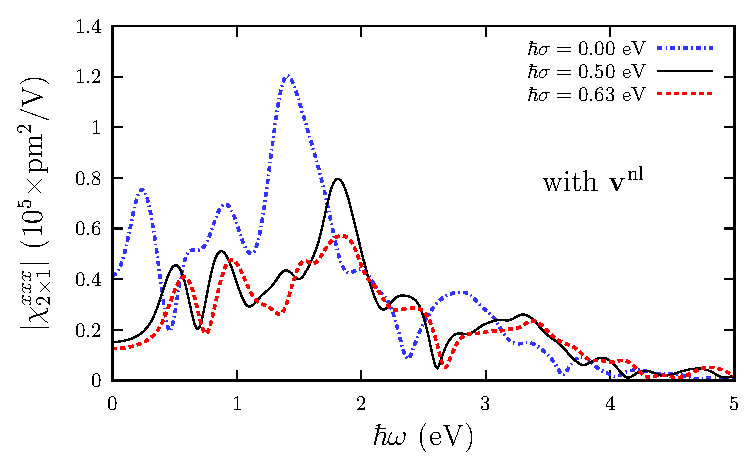
\includegraphics[scale=.8]{plots/fig4}
\caption{(color on line) 
$\chi^{xxx}_{2\times 1}$
vs $\hbar\omega$ for a slab with 32 
atomic Si layers plus one H layer, 
for two different values of 
the scissors correction $\hbar\Delta$. 
\label{fig4}} 
\end{figure}
